\documentclass[10pt,a4paper]{article}

\usepackage{listings}
\usepackage{graphicx}
\usepackage{float}
\usepackage[margin=0.5in]{geometry}
\usepackage{amsmath}
\usepackage{enumitem}% http://ctan.org/pkg/enumitem
\usepackage{etoolbox}


\usepackage{tcolorbox}
\usepackage[hidelinks]{hyperref}
\usepackage{array}
\usepackage{tabularx}
\AtBeginEnvironment{tabularx}{\scriptsize}
\renewcommand{\tabularxcolumn}[1]{m{#1}}
\setlist{nolistsep}
\setlist{nosep}
\newcommand{\cbox}[2]{
    \begin{tcolorbox}[title=#1,
        colback=red!5!white,
        colframe=red!50!black,
        size=fbox,
        % left=2mm,
        % right=3mm,
        fonttitle=\bfseries]
        #2
    \end{tcolorbox}
}




\DeclareMathOperator*{\argmax}{arg\,max}
\DeclareMathOperator*{\argmin}{arg\,min}

\begin{document}



\pagenumbering{Roman}
% \tableofcontents
% \newpage
\pagenumbering{arabic}


\section{Software Architecture}
The solution is divided into four main components: 
\begin{itemize}
    \item The \textbf{client} - responsible for interfacing with the server or other methods of data input
    \item The \textbf{pathfinding} module - handling graph search and pathing between two points in any space
    \item The \textbf{simulation} module - handling the route selection and the actual "drone control" with the use of pathfinding
    \item The \textbf{visualisation} module - responsible for generating visualisations of the output from the simulation module
\end{itemize}

Most of the inter-module design choices explained below, are fueled by the dependency inversion principle and the rest by good general OOP practice. 
Due to the size of the solution, a lot of the simpler classes are missed out of the diagrams. 
The descriptions below will revolve mostly around the key decisions in the architecture and their benefits.

\subsection{Client module}
Figure \ref{fig:client} shows the structure of the client module classes, it contains Data classes which hold the intermediate, validated and standardised data.
These intermediate classes detach the implementation from the exact shape input data. 
Since any number of formats can map to these classes, the solution is not closely related to the input data - this is very desirable. \par

The ClientService interface is used to actually create the data in the form of Data classes from the input data given. 
In the case of AQmaps the data is given via http server and so an appropriate implementing class will need to know the base URI/location of the API where sensor/map/w3w data is stored, and have access to the Http protocol.

\par 
Any other classes which will "feed" into the rest of the system, but are constructed from input data, will be declared in this module and implement the appropriate external service interfaces.

\begin{figure}[h]
    \centering
    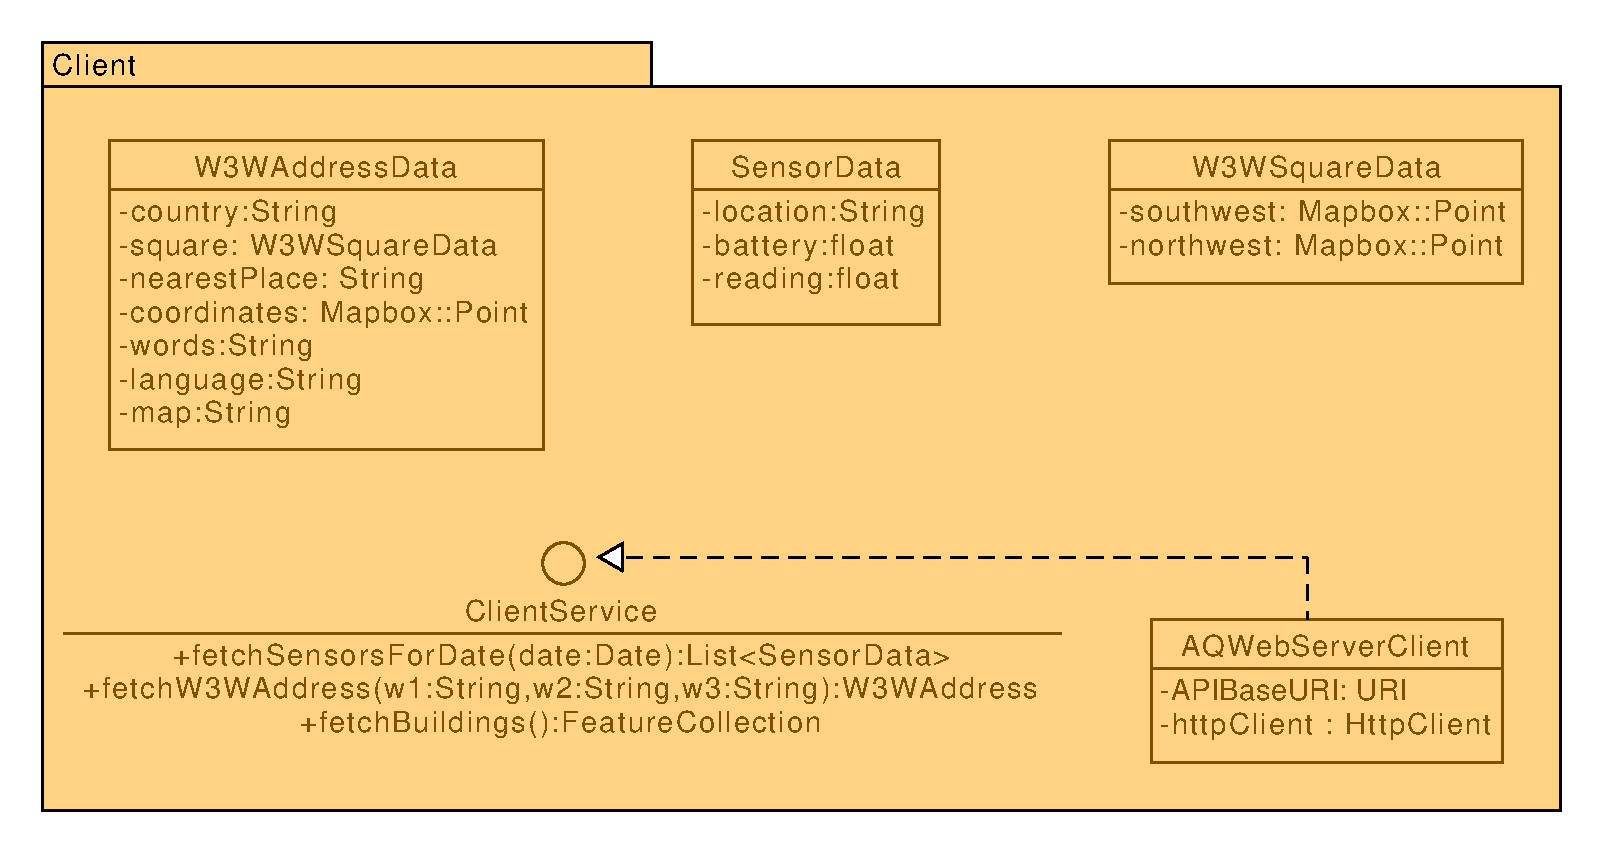
\includegraphics[width=0.7\columnwidth]{diagrams/client.uxf.pdf}
    \caption{UML diagram of the client module}
    \label{fig:client}
\end{figure}

\subsection{Pathfinding module}
We separate the problem of pathfinding completely from the AQmap problem. This allows a broader range of techniques to be applied much more easilly.
\par 
\medskip
Figure \ref{fig:pathfinding} shows the most important classes from the pathfinding module. 
The basis of this module is formed by the SearchNode and PathfindingAlgorithm abstract classes as well as the Graph interface.
\par
The PathfindingAlgorithm class defines an abstract findPath method for finding a path to a single goal, leaving the exact way this is done to the concrete implementation. 
It is marked as abstract since we will always need to apply pathfinding to multiple goals as well, and so this class should deal with that, since this would otherwise always have to be done by the consumer.
\par
Each SearchNode is used to represent a part of the frontier of a graph search algorithm i.e. a \textbf{state} in the search space - in the pathfinding case, a path. 
These are made abstract to allow for the use of generics in such a way that each parent node is of the specific node type needed and also because nodes are expected to be annotated with problem specific data.
It is this generic parameter which propagates to the rest of the classes.
\par
Due to the fact we are mostly dealing with multiple goal pathfinding, each node should also hold a deque of goals which can be reached from it - take as an example the problem where you start at a position with 2 goals, no movement is necessary and both are reached.
\par
Pathfinding goals are represented by their own class, alternatively we could simply use coordinates as goals, 
but this would force the consumer of this functionality to always have to match the coordinates of the path returned to the goals that it needed achieved,
as opposed to simply looking through the goals achieved by each node and comparing them via reference to the deque of goals in order.

\par 
Finally the Graph interface defines the transition function from any searchNode to all its neighbours. 
PathfindingAlgorithms always accept the graph as a parameter as it forms the domain of each specific problem. 
Separating the domain from the algorithm completely makes the algorithms much more flexible and easier to unit test.

\par 
Other interfaces shown include the SpatialHash and PathfindingHeuristic, those will be used by implementing algorithms and are defined as interfaces 
to again further separate the components of algorithms from the domain. This allows us to further change the behaviour and performance of algorithms,
by swapping out their components to suit (Composition over Inheritance). 





\subsection{Simulation module}
The simulation module is responsible for: planning the route (using TSP solvers), applying pathfinding to find the detailed path required for collection, and setting the read status in sensors. 
The name stems from the fact that our sensor data collection is only simulated. This module directly interfaces with the pathfinding module as expected. 
Principles of dependency inverersion were applied to reduce coupling and increase flexibility.
\par 
\medskip
Figure \ref{fig:simulation} shows the most important classes of the simulation module. The biggest architectural choice here is the splitting of the drone into components. 
\\
This means that we keep the specific pathfinding and route planning behaviour separate from the behaviour of the drone/data collector itself.
Since it is not the job of the path or route planner to "read" any sensors, this will be the task of the drone in addition to perhaps applying some strategy
to the produced path in case it is not satysfying enough (maybe re-routing from a point with a different collection order).
\par
Another big choice is the fact that this module does not know anything about the input data, it simply defines a contract for the sensor class, letting the consumers of this module deal with 
data conversion.

\par 
The path planner component itself is further composed of the PathfindingAlgorithm and DistanceMatrix which means it only concerns itself with the 
task of translating a path of individual points it receives from the PathfindingAlgorithm to a path composed of path segments enforcing the move pattern of the drone.
\par
The PathSegment class is necessary since it is a major requirement that the collector must move in a specific pattern, this class can be used to enforce such a contract.
\par 
On the other hand CollectionOrderPlanners are only defined by their implementation and the choice of DistanceMatrix as well as the set of route optimisers. 
This choice decouples the major TSP solving strategy from the distance measure that it uses. 
\par
Both the PathPlanner and CollectionOrderPlanner interfaces have a base abstract class implementation since:
\begin{itemize}
    \item Collection order planners will always apply the set of given optimisers to the final route.
    \item They will also have to always set up the distance matrix with the given sensors 
    \item Path planners will always have to apply the given pathfinding algorithm before actually performing conversion to path segments
    \item We also use these abstract bases to enforce problem specific rules, such as the maximum number of moves, this leaves the possibility of
            straying away from those base classes if the problem changes drastically in the future.
\end{itemize}
\par 
This module also implements a specific Graph and SearchNode specific to the problem at hand. Here the ConstrainedTreeGraph produces nodes satisfying 
the angle, move length and obstacle constraints, in effect all logic to do with checking whether the collector is hitting an obstacle, or if the move length is valid etc.. is contained 
in the graph itself. This is very desirable and intentional. 
The addition of the direction field to the DirectedSearchNode further emphasizes the angle requirements, and allows for the construction of 
PathSegments from search nodes without calculating angles twice.
\par Another important class here is the abstract Sensor class. This is made abstract for two reasons:
\begin{itemize}
    \item The concrete implementation of the sensor should be done in another module, since it is more convenient for example to closely link it 
        to the input data for convenience. So according to the principle of dependency inversion we do not provide a concrete implementation in this module.
    \item The sensor cannot show any reading unless it is actually read, this can be enforced by this abstact class using the setHasBeenRead method regardless of the 
        concrete implementation/constructor.
\end{itemize}




\subsection{Visualisation module}
This module only needs to interface with the output classes of the simulation module, i.e. the PathSegment and Sensor classes but other than that, it is 
completely decoupled from the shape of the initial input data of the system. This is very desirable 
\par
Figure \ref{fig:visualisation} shows the UML diagram of the most important classes in the visualisation module.
\\
Classes implementing the SensorCollectionVisualiser interface generate geojson visualisations of sensor data collections.
These have access to both the flight path and the sensors and hence their readings. The AQMapGenerator is the problem specific example of implementation of such a visualiser.
\par
Using an interface like like this allows for the swapping out of visualisers at will whenever new requirements arise or current ones change.
\par 
The OutputFormatter class deals with writing the visualisations and flight paths to a file, these are made static as changes in output format are assumed to be very few in the future,
and should such changes be required, new methods can be added to the formatter.
\par 
The usage of the AttributeMap interface allows for a lot of flexibility in the way the AQMapGenerator assigns colors and symbols, and should this behaviour need to be changed, it'd be very easy to do.
\begin{figure}[H]
    \centering
    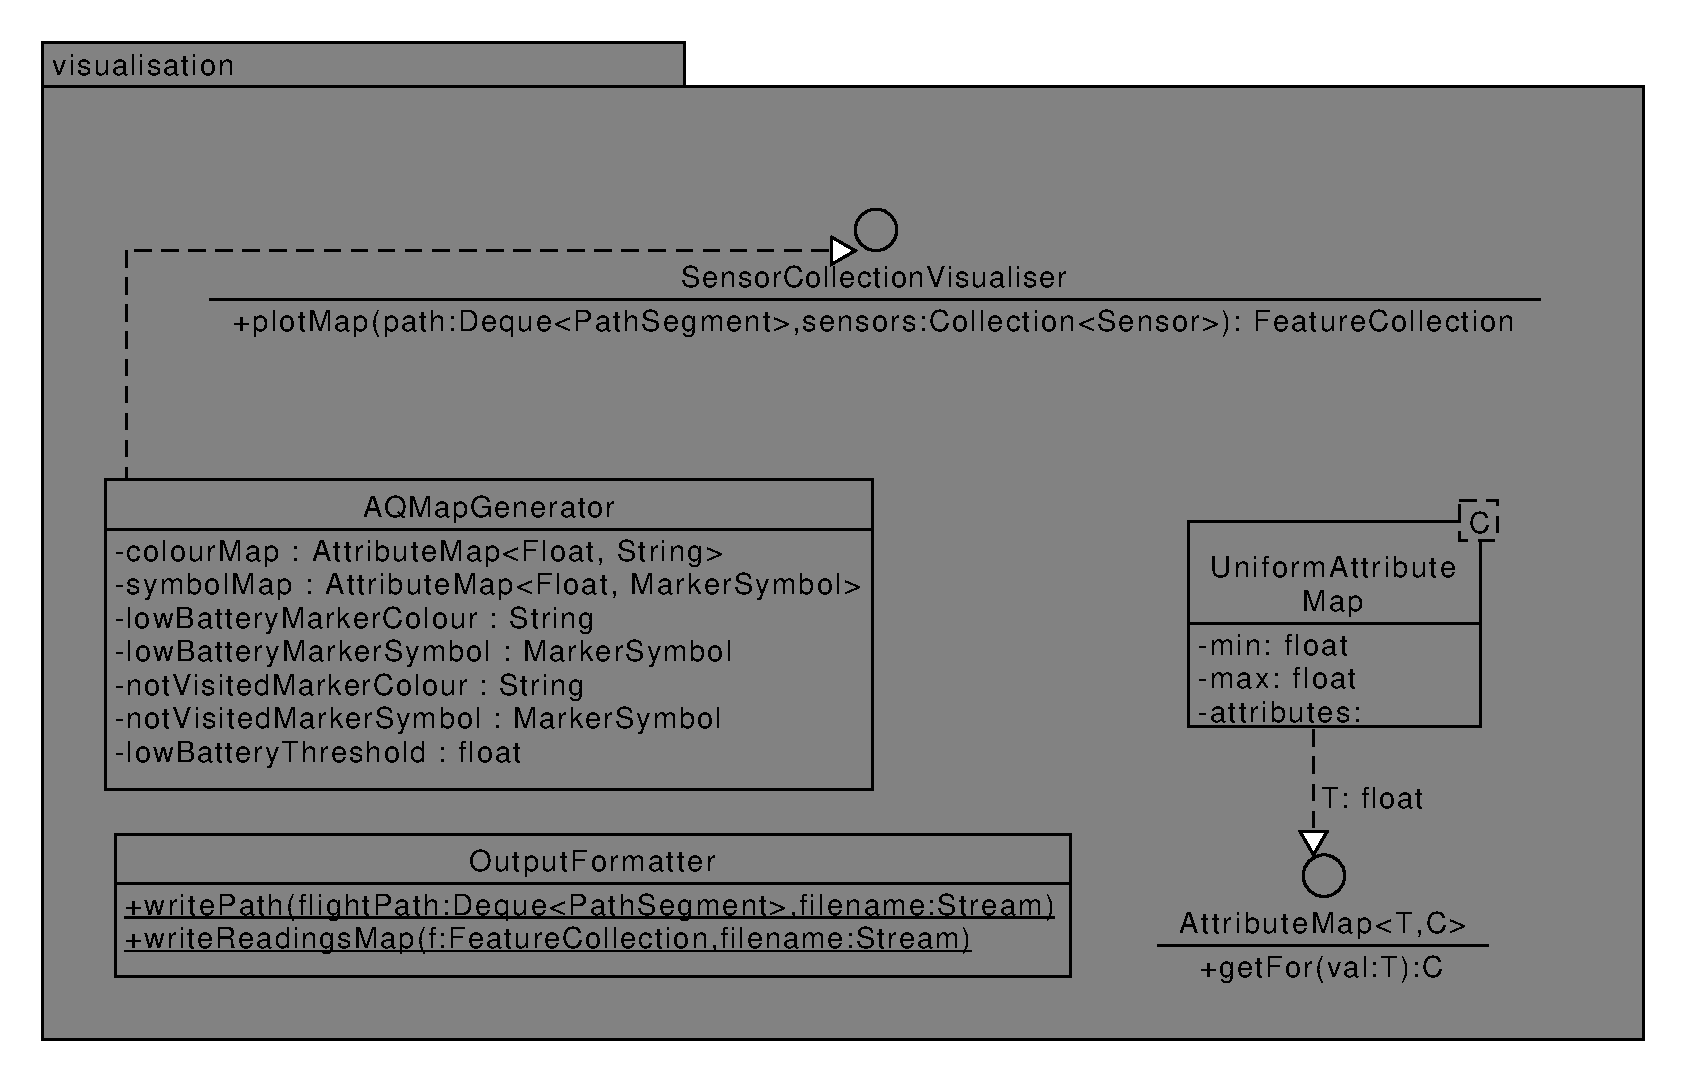
\includegraphics[width=0.7\columnwidth]{diagrams/visualisation.uxf.pdf}
    \caption{UML diagram of the Visualisation module}
    \label{fig:visualisation}
\end{figure}
\begin{figure}[H]
    \centering
    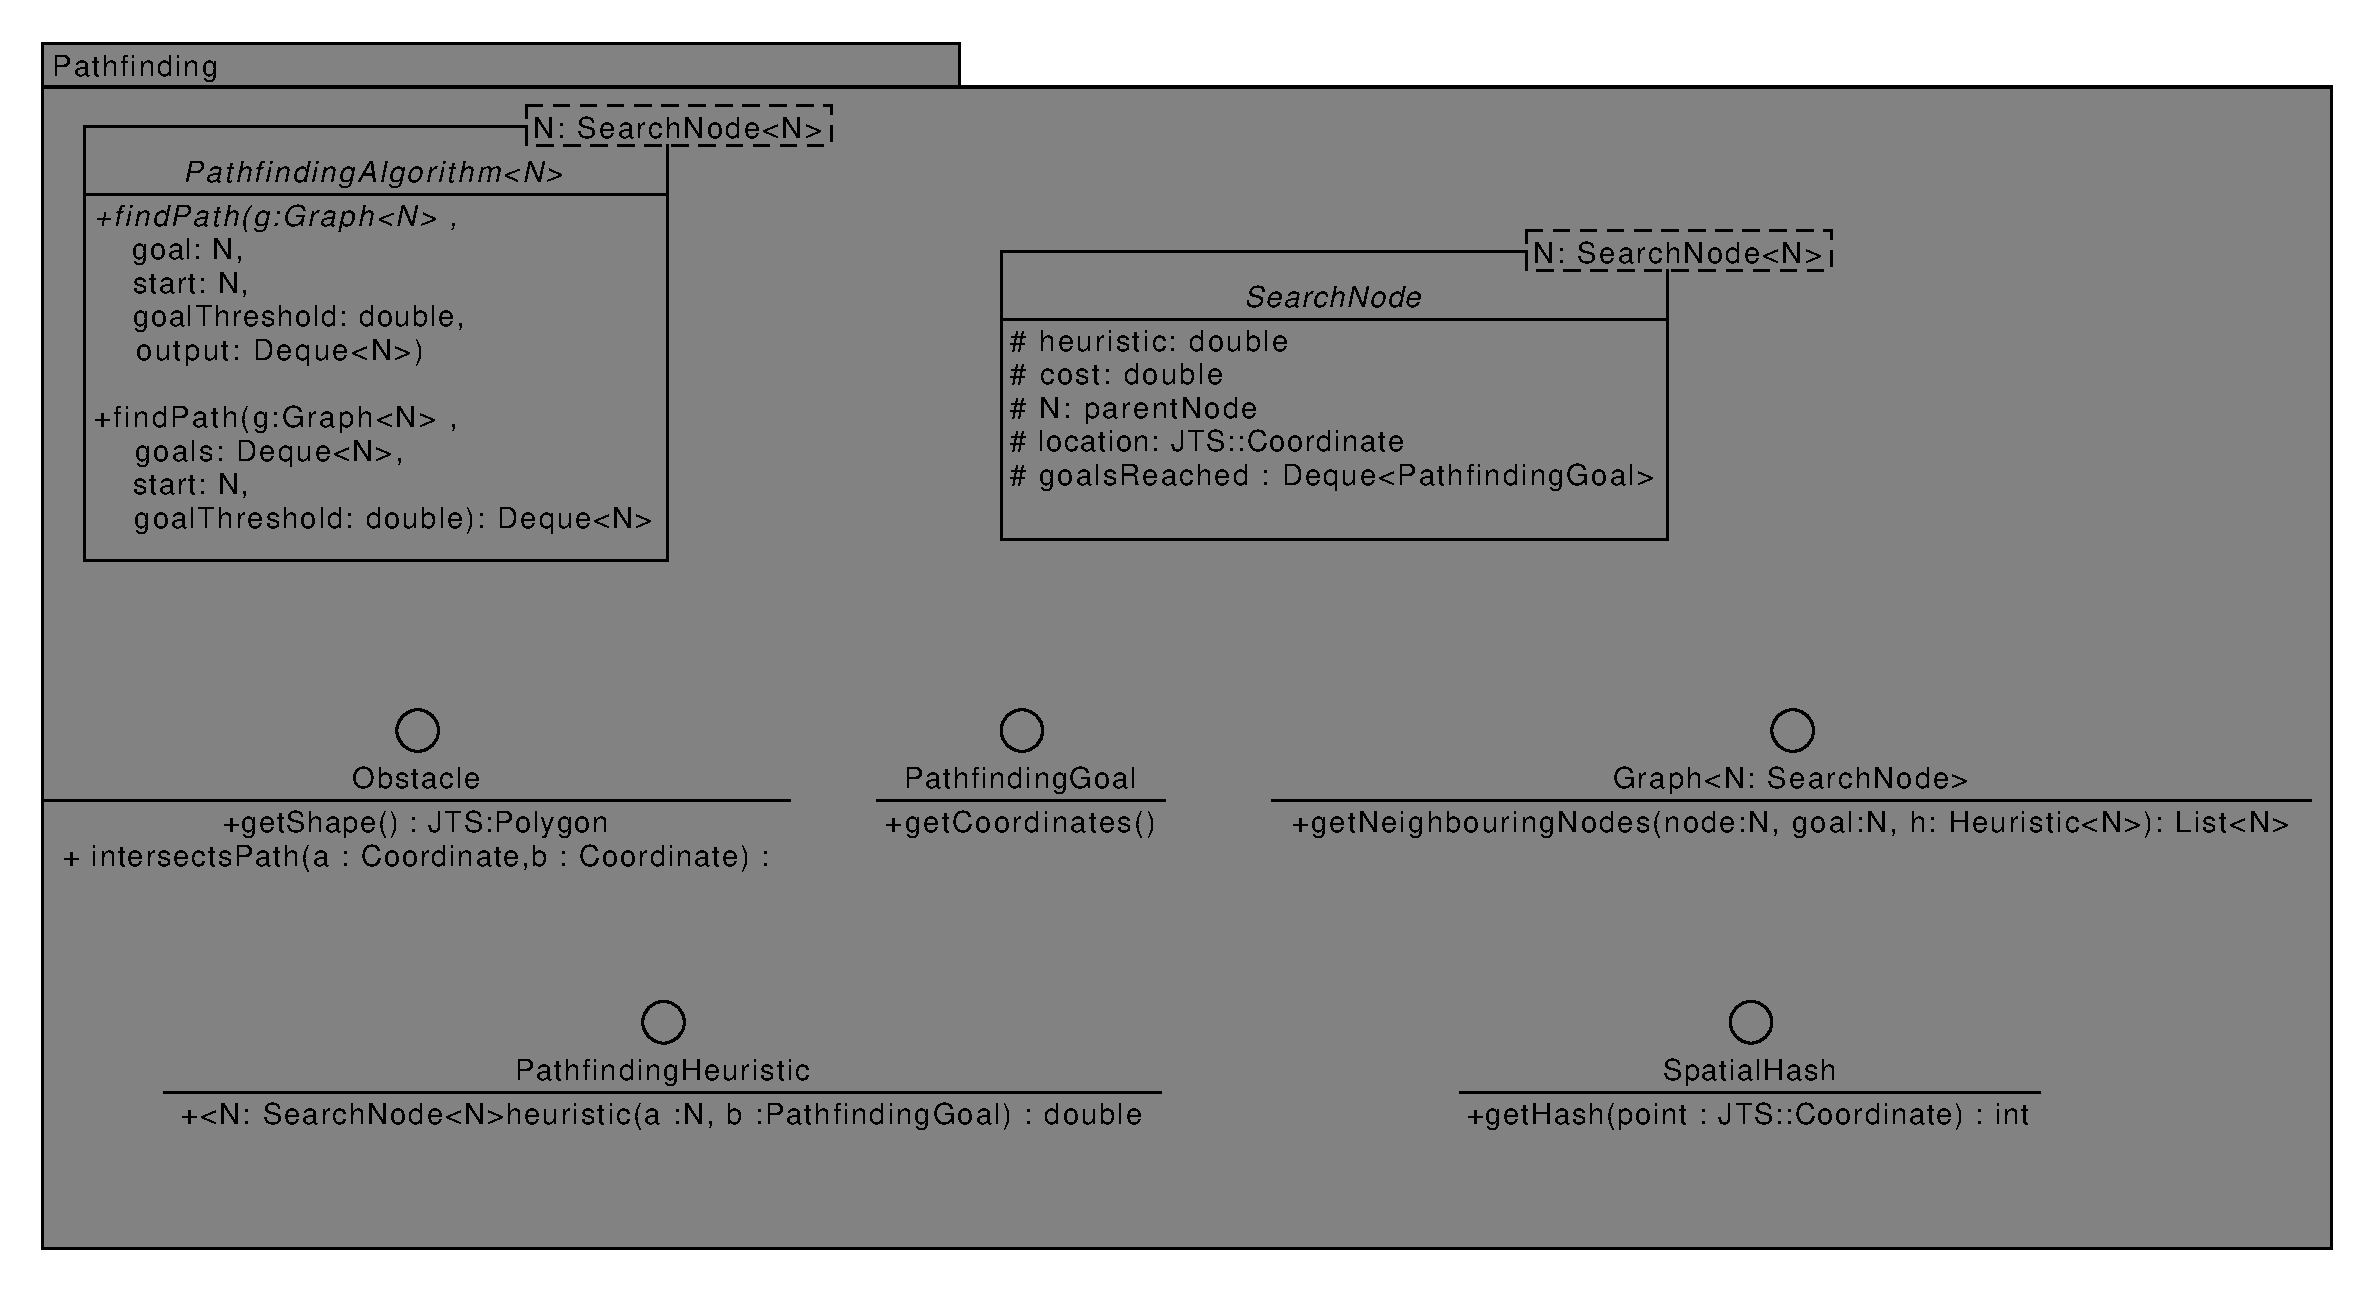
\includegraphics[width=0.7\columnwidth]{diagrams/pathfinding.uxf.pdf}
    \caption{UML diagram of the pathfinding module}
    \label{fig:pathfinding}
\end{figure}
\begin{figure}[H]
    \centering
    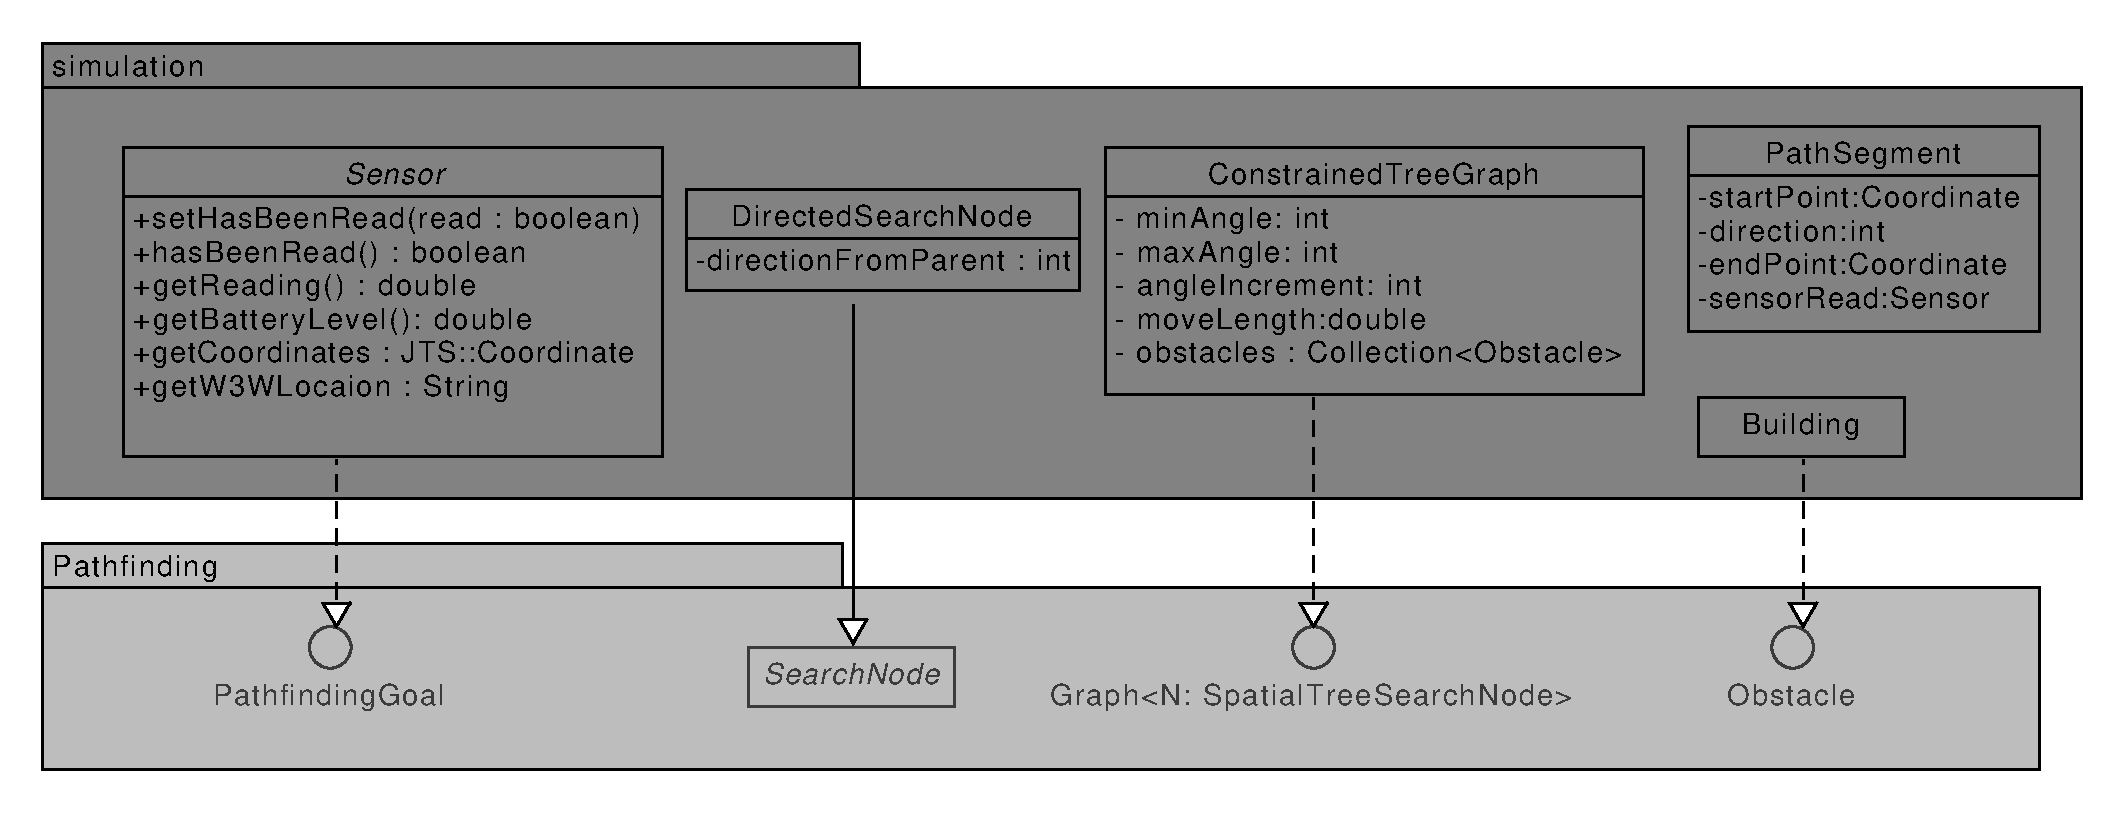
\includegraphics[width=0.8\columnwidth]{diagrams/simulation.uxf.pdf}
    \caption{UML diagram of the Simulation module}
    \label{fig:simulation}
\end{figure}

\section{Drone Control Algorithm}
\subsection{TSP Solver}

\lstdefinestyle{mystyle}{
    % backgroundcolor=\color{backcolour},
    % commentstyle=\color{codegreen},
    % keywordstyle=\color{magenta},
    % numberstyle=\tiny\color{codegray},
    % stringstyle=\color{codepurple},
    basicstyle=\footnotesize,
    % breakatwhitespace=false,
    % breaklines=true,
    % captionpos=b,
    % keepspaces=true,
    % numbers=left,
    % numbersep=5pt,
    % showspaces=false,
    % showstringspaces=false,
    % showtabs=false,
    % tabsize=2,
    % numberfirstline=false,
    mathescape,
    literate=
        {=}{$\leftarrow{}$}{1}
        {==}{$={}$}{1}
        {!=}{$\neq$}{1}
        {leq}{$\leq{}$}{1}
        {nullset}{$\emptyset$}{1}
        {geq}{$\geq{}$}{1},
    morekeywords={Let,While,ArgMax,ArgMin, Function, For, If, return, Return, Algorithm, Skip},
}

\begin{figure}[H]
    \begin{lstlisting}[style=mystyle]
        Algorithm NearestInsertion:
            Let R be the sensor nearest to the starting point
            Let U = unvisited sensors
            Let T = [R] be the current tour (implicitly looping)

            While U != nullset:
                R = $\argmin_{s\in R}$ distanceToTour(s) 
                i = $\argmin_{i\in I(T)}$ insertionCost(i,R)
                T = T with R inserted at i
                U = U - {R}
            
            Return T

        Function distanceToTour(s):
            minimum = $\infty$
            For t in T:
                If dist(s,t) < minimum:
                    minimum = dist(s,t)
            Return minimum
        
        Function insertionCost(i,s):
            N = T with s inserted at i
            Return euclidian length of N
        

    \end{lstlisting}
    \caption{Nearest Insertion TSP solver}
    \label{alg:ni}
\end{figure}

The choice of which order to visit the sensors in is a general TSP problem.
\par 
The heuristic chosen to tackle this part of the problem was the \hyperref[tab:NearestInsertionCollectionOrderPlanner]{\color{blue}Nearest Insertion heuristic} followed by a number of \hyperref[tab:Optimiser2Opt]{\color{blue}2-opt optimisations}.
\par
As pseuducode in Figure \ref{alg:ni} shows, the heuristic inserts sensors into the tour one at a time, choosing the sensor which is closest to any sensor in the tour.
\\
After a route is found, 2-opt optimisations are applied to it to remove paths which are crossing each other.
The 2-opt algorithm in each pass checks if reversing any sub-segment of all possible sub-segments of a full tour reduces it's cost, and if so keeps the reversal. 
The passes are repetead until improvements fall under a threshold of 0.00003 degrees

This alrogithm turns out to be pareto-optimal \cite{metric-tsp} among a family of cutting-edge algorithms for problem sizes of between 30-50 vertices.
Pareto-optimality means that this algorithm was either finding the best path compared to the other algorithms, or was finding one the quickest. 
Since this process yields the route built on the Minimum Spanning Tree, 
the path found will always be less than or equal to 2 times the optimal solution \cite{2-approximation-ni}.
\subsection{Generating neighbour nodes}
All the other sections of the algorithm make use of the "neighbour" function, i.e. the function which generates neighbour nodes for any node representing 
a point on the map.

This is done using the \hyperref[tab:BVHNode]{\color{blue}{Bounding Volume Hierarchy}} data structure. 
The structure allows for logarithmic time lookups of possibly colliding obstacles (with any shape).
We do this by creating a binary tree whose nodes are defined by an Axis Aligned Bounding Volume enveloping all the obstacles present in the leaf nodes underneath the node.
The root node then envelops all the obstacles present in the hierarchy.
\par
When creating the tree we find the axis along which the difference between the extremal coordinates of the AABB's is the largest, i.e. the "longest axis".
We then pick a splitting point on the axis and partition the shapes into the left and right sub trees according to which side of the splitting point they're on.
\par 
With this setup, the structure can tell us which obstacles are possibly colliding with any given shape by checking for collisions (cheaply) with the AABB's and only returning those leafs whose AABB's were collided with (possibly from both subtrees).

\subsection{Pathfinding}
\begin{figure}[H]
    \begin{lstlisting}[style=mystyle]
        Algorithm A*:
            Let R = starting node
            let G = goal coordinates
            Let O = {R} // open set
            Let V = {} // approximately visited
            
            While O != nullset:
                R = $\argmin_{o\in O}$ Fvalue(o)
                O = O - R

                If isNearGoal(R):
                    R.goalsReached = R.goalsReached + G
                    Return reconstructPath(R) // using parent references

                // generate neighbour nodes with appropriate costs and parent set to R
                // nodes colliding with obstacles or outside of boundary are excluded
                // this is done via Bounding Volume Hierarchies
                N = neighbours(R) 

                For n in N:
                    
                    hash = cantorHash(n.x,n.y)

                    If hash in V:
                        Skip n
                    
                    V = V + hash
                    O = O + n
            
            // no path found
            Return []

        Function Fvalue(n):
            Return dist(n,G)*1.5 + cost(n)

        Function cantorHash(x,y):
            Let gridWidth = $\frac{1}{75} * 0.0003 $
            Let gridX,gridY = coordinates of center of drone confinement area 
            nx,ny = (x - gridX)/gridWidth,(y - gridY)/gridWidth
            nx,ny = makePositive($\lfloor nx \rfloor$),makePositive($\lfloor ny \rfloor$)

            return $\lfloor$(((0.5 * (nx + ny)) * (nx + ny + 1)) + ny)$\rfloor$;
        
        Function makePositive(n):
            If n $\geq$ 0:
                Return $2n$
            Otherwise:
                Return $-2n - 1$
               
            
            
    \end{lstlisting}
    \caption{Custom A* pathfinding algorithm}
    \label{alg:a*}
\end{figure}

Pathfinding between any two points on the plane was carried out using the \hyperref[tab:AstarTreeSearch]{\color{blue}A* tree search} algorithm using the euclidian distance heuristic. 
The algorithm is just a modified breadth-first search, where the search nodes are picked in order of least f value which is defined as:
    $f(n) = 1.5 \cdot h(n) + c(n)$
with $c(n)$ being the cost of reaching the node n from the start state, and $h(n)$ is the approximation of the cost of reaching the goal state from the node n.
\\

\noindent The heuristic is relaxed by a factor of 1.5, to promote the expansion of straighter paths.
\noindent This means that the paths are no longer optimal as the heuristic is no longer admissible, but since most paths would not be obstucted by buildings - this
change does not actually impact the length of the paths all that much.

To speed up the algorithm \hyperref[tab:GridSnappingSpatialHash]{\color{blue}spatial hashing} was used to prune nodes which were visited (or visited close-enough), expressing their coordinates relative to a grid centered around the center of the boundary (with integer width square size), and hashing those coordinates
using a modified cantor pairing allowing for negative values.

\subsection{Path segmenting}
Once we have a path of individual points, we need to convert it to a path of path segments with information about which sensor is read at each segment.
We can do this by "sliding" a window over the points and always looking at two points at a time in order. 
We call the points at each position of the windo P and N, where P is the point before N. 
The pathfinding algorithm also attaches a deque of sensors reached by each P/N.  
A naive sequential pairing does not work due to multiple goals allowed at each point, and the requirement of the drone to move before collecting the reading.
We apply a number of rules to make a valid path:

\noindent (portrayed in Figure \ref{fig:segmenting}):
\begin{itemize}
    \item While P attains a goal, create a proxy segment to any neighbouring node, and one back, assign the first sensor attained by P 
        to the newest back-facing segment's N node
    \item If N attains no goals, see if the next segment's P node attains any sensors, if so "steal" one away from it
    \item while N attains more than one sensor reduce the number of attained sensors by creating proxy segments as above for each
    \item If N only attains one sensor or none, create P-N path segment as normal
\end{itemize}

\begin{figure}[H]
    \centering
    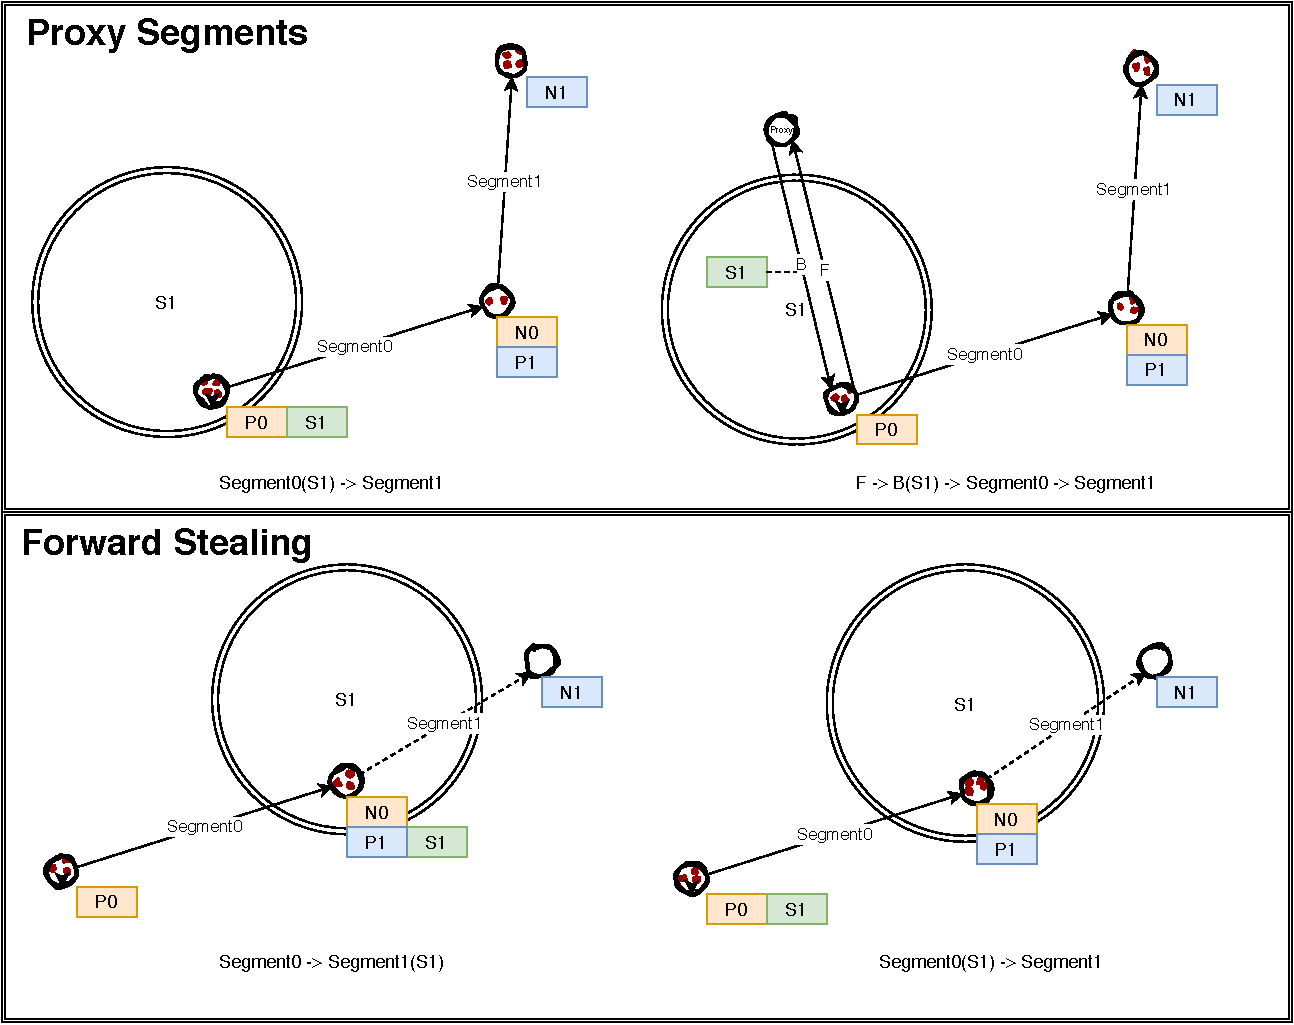
\includegraphics[width=0.7\columnwidth]{diagrams/diagram.pdf}
    \caption{Segmenting behaviours}
    \label{fig:segmenting}
\end{figure}

\subsection{Examples}
The algorithm was tested on over 35000 configurations over the data provided. 
The hardest and easiest collection days' geojson visualisations are shown below (with the algorithm set to optimal parameters as given above) 
\begin{figure}[H]
    \centering
    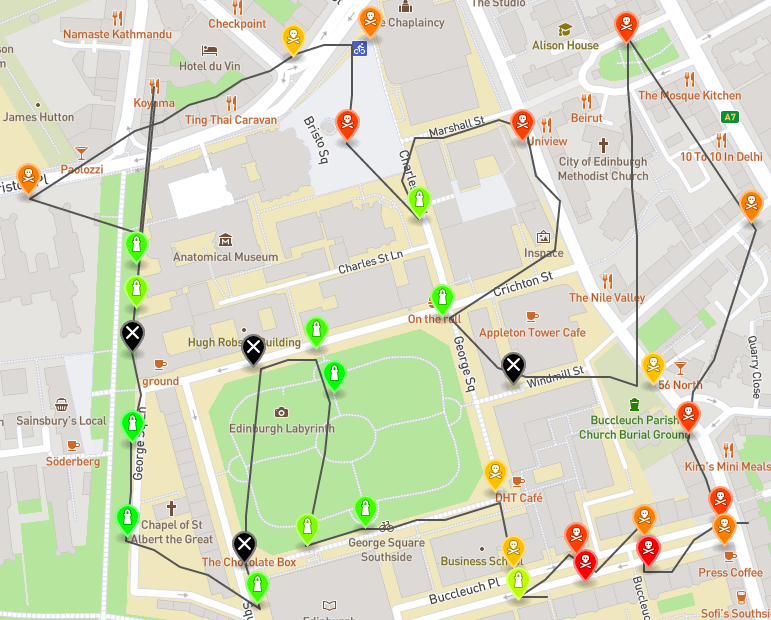
\includegraphics[width=0.4\columnwidth]{diagrams/hard-day.png}
    \caption{geojson.io rendering of hardest collection at day 9-2-2020 with a starting point of -3.19087,55.945778, with 111 moves}
    \label{fig:hardmap}
\end{figure}
\begin{figure}[H]
    \centering
    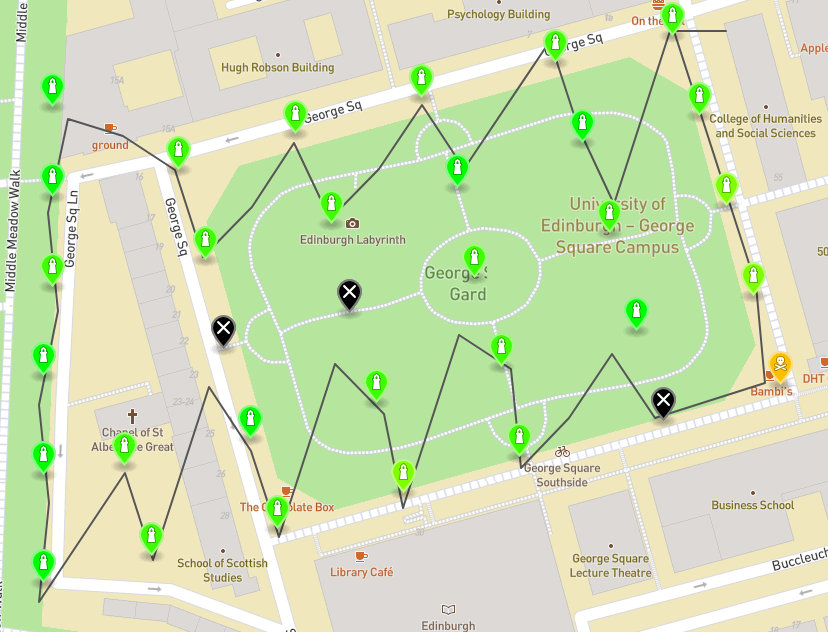
\includegraphics[width=0.4\columnwidth]{diagrams/easy-day.png}
    \caption{geojson.io rendering of easiest collection at day 2-1-2021 with a starting point of -3.1878,55.9444, with 46 moves}
    \label{fig:easymap}
\end{figure}

The artifacts of path segmenting are evident in the harder day, where the drone wanders near closely spaced sensors on the bottom right it creates a horizontal 
proxy segment. But overall the algorithm manages very well, never carrying out the collection in more than 111 moves and averaging at 90 moves $\pm$ 6.7. Execution times averaged at 103ms.

\section{Class Documentation}

\subsubsection{ .ac.ed.inf.aqmaps.visualisation }
\subparagraph{ AttributeMap } Attribute maps divide their domain into attribute buckets and allow for quick retrieval of the necessary attributes
 
\hrule
\begin{mitem}
\scriptsize
	\mitemxx{ \textbf{ C getFor  } (T o)}
	{Retrieve attribute for the given input}
\end{mitem}

\subparagraph{ MarkerSymbol } Available symbols for use with geojson
 
\hrule

\subparagraph{ SensorCollectionVisualiser } Classes implementing this interface generate geojson visualisations of the flight path and sensor readings
 
\hrule
\begin{mitem}
\scriptsize
	\mitemxx{ \textbf{ com.mapbox.geojson.FeatureCollection plotMap  } (Deque<PathSegment> flightPathCollection<Sensor> sensorsToBeVisited)}
	{Create a geojson visualisation of the given flight path and sensors with their readings}
\end{mitem}

\subparagraph{ UniformAttributeMap } A general attribute map which maps a range of values from a (min,max) range to attribute buckets of size (max-min)/buckets number uniformly.
 
Implements \textbf{ AttributeMap }
\hrule
\begin{mitem}
\scriptsize
	\mitemxx{ \textbf{ public UniformAttributeMap  } (Float minFloat maxC... attributes)}
	{}
	\mitemxx{ \textbf{ public C getFor  } (Float value)}
	{Retrieve attribute for the given input}
\end{mitem}

\subsubsection{ .ac.ed.inf.aqmaps.utilities }
\subparagraph{ BVHNode } Bounding Volume Hierarchy Node. This class forms a tree of AABB (Axis aligned bounding boxes) for internal nodes
 and of any shapes at the leaf nodes. Allows for quick broad phase collision checks between objects. Will never return a false negative but might return
 false positives. I.e. this structure only tells you which objects are possibly colliding (whose AABB's intersect).
 
\hrule
\begin{mitem}
\scriptsize
	\mitemxx{ \textbf{ public BVHNode  } (Collection<T> shapes)}
	{Construct a new bvh hierarchy with the given shapes at the leaf nodes}
	\mitemxx{ \textbf{ public Collection<T> getPossibleCollisions  } (org.locationtech.jts.geom.Geometry other)}
	{Retrieves all possibly coliding objects (their bounding boxes intersect) from within the tree.}
\end{mitem}

\subparagraph{ GeometryFactorySingleton } The geometry factory containing the precision model to be used when generating geometries with JTS
 
\hrule
\begin{mitem}
\scriptsize
	\mitemxx{ \textbf{ public GeometryFactorySingleton } ()}
	{}
	\mitemxx{ \textbf{ public static org.locationtech.jts.geom.GeometryFactory getGeometryFactory } ()}
	{Retrieve the geometry factory, containing the precision model}
\end{mitem}

\subparagraph{ GeometryUtilities } A collection of utility geometry methods
 
\hrule
\begin{mitem}
\scriptsize
	\mitemxx{ \textbf{ public GeometryUtilities } ()}
	{}
	\mitemxx{ \textbf{ public static org.locationtech.jts.geom.Coordinate MapboxPointToJTSCoordinate  } (com.mapbox.geojson.Point p)}
	{Convert a mapbox point to a jts coordinate}
\end{mitem}

\subparagraph{ MathUtilities } 
 
\hrule
\begin{mitem}
\scriptsize
	\mitemxx{ \textbf{ public MathUtilities } ()}
	{}
	\mitemxx{ \textbf{ public static double angleFromEast  } (org.locationtech.jts.math.Vector2D a)}
	{returns the angle from the eastern direction clockwise between 0 and 360 of the vector}
\end{mitem}

\subparagraph{ Shape } Anything which contains a shape can implement this interface. Shapes can be polygons, or absolutely any other geometry
 
\hrule
\begin{mitem}
\scriptsize
	\mitemxx{ \textbf{ org.locationtech.jts.geom.Geometry getShape } ()}
	{Return this shape's geometry}
\end{mitem}

\subsubsection{ .ac.ed.inf.aqmaps.simulation.planning.path }
\subparagraph{ BasePathPlanner } Base class for planners with a limited number of maximum moves and a
 minimum reading range. All inheriting path planners must make sure that each sensor is read at the endpoint of some path segment
 and that that sensor is within reading range of the endpoint. They also must make sure that the path is under the maximum move limit
 
Implements \textbf{ PathPlanner }
\hrule
\begin{mitem}
\scriptsize
	\mitemxx{ \textbf{ public BasePathPlanner  } (double readingRangeint maxMovesPathfindingAlgorithm<DirectedSearchNode> algorithm)}
	{}
	\mitemxx{ \textbf{ public Deque<PathSegment> planPath  } (org.locationtech.jts.geom.Coordinate startCoordinateDeque<Sensor> routeConstrainedTreeGraph graphboolean formLoop)}
	{Plans the exact path required to reach all the given sensors, the specific constraints on placed on the route are decided\newline%
 by the specific implementation of the planner itself.\newline%
 The ConstrainedPathPlanner class adds a maximum move,reading range and also the move sequence constraint to the path planning problem, a valid path will allow the collector\newline%
 to come within READING\_RANGE of each sensor (the distance between each sensor and the collector at some path segment's endpoint will be less than or equal to READING\_RANGE).\newline%
 The number of segments returned will always be <= MAX\_MOVES. The move sequence in each path segment requires that a sensor be read at the end of each path segment only, i.e. the collector must move before collecting\newline%
 any reading, and only one reading must be made per path segment.}
\end{mitem}

\subparagraph{ PathPlanner } Path planners create a detailed path between given route points which takes a sensor data collector 
 between the route points according to the path planner's constraints
 
\hrule
\begin{mitem}
\scriptsize
	\mitemxx{ \textbf{ Deque<PathSegment> planPath  } (org.locationtech.jts.geom.Coordinate startCoordinateDeque<Sensor> routeConstrainedTreeGraph graphboolean formLoop)}
	{Plans the exact path required to reach all the given sensors, the specific constraints on placed on the route are decided\newline%
 by the specific implementation of the planner itself.}
\end{mitem}

\subparagraph{ PathSegment } represents a singular move made by the sensor data collector
 each move follows the pattern of: move->collect reading, 
 we cannot collect a reading in a move unless we have moved
 
\hrule
\begin{mitem}
\scriptsize
	\mitemxx{ \textbf{ public PathSegment  } (org.locationtech.jts.geom.Coordinate startPointint directionorg.locationtech.jts.geom.Coordinate endPointSensor sensorRead)}
	{Creates a path segment from the start and end points, the direction of movement and the sensor read if any}
	\mitemxx{ \textbf{ public org.locationtech.jts.geom.Coordinate getStartPoint } ()}
	{}
\end{mitem}

\subparagraph{ SimplePathPlanner } This path planner will apply some simple optimisations in order to produce a smaller number of path segments than the naive implementation.
 
Implements \textbf{ PathPlanner }
\hrule
\begin{mitem}
\scriptsize
	\mitemxx{ \textbf{ public SimplePathPlanner  } (double readingRangeint maxMovesPathfindingAlgorithm<DirectedSearchNode> algorithm)}
	{}
	\mitemxx{ \textbf{ protected Deque<PathSegment> pathPointsToSegmentsStrategy  } (Deque<DirectedSearchNode> pathPointsDeque<PathfindingGoal> goalsRouteDeque<Sensor> sensorRouteConstrainedTreeGraph graph)}
	{The main defining characteristic of a constrained path planner. Converts a path of points to a path of path segments\newline%
 needs to make sure that each pathfinding goal is visited only in the end segment of some path segment in range.\newline%
 the passed deque arguments will be consumed. This planner will try to perform some simple optimisations in order to shorten the route.\newline%
 In order to produce a valid route this planner will introduce proxy segments which go back and forth between the nearest neighbour\newline%
 whenever a sensor is read at the start point of a segment or if more than one sensor is read at the endpoint. The optimisations currently include:\newline%
  \newline%
 1) if the current segment does not read anything at the end point and the next reads a sensor at its start point, we "absorb" that sensor into\newline%
 the current segment.}
\end{mitem}

\subsubsection{ .ac.ed.inf.aqmaps.simulation.planning.collectionOrder.optimisers }
\subparagraph{ CollectionOrderOptimiser } Collection order optimisers provide re-usable methods for optimising a route after one is already selected
 
\hrule
\begin{mitem}
\scriptsize
	\mitemxx{ \textbf{ void optimise  } (DistanceMatrix distanceMatrixint{[}{]} path)}
	{}
\end{mitem}

\subparagraph{ Optimiser2Opt } An optimiser which performs the 2-opt algorithm to remove crossings in the path
 
Implements \textbf{ CollectionOrderOptimiser }
\hrule
\begin{mitem}
\scriptsize
	\mitemxx{ \textbf{ public Optimiser2Opt  } (double epsilon)}
	{Construct a 2 opt optimiser with the given epsilon threshold. The threshold determines the minimum decrease in path cost required for the optimiser to keep optimising each loop.}
	\mitemxx{ \textbf{ public void optimise  } (DistanceMatrix distanceMatrixint{[}{]} path)}
	{}
\end{mitem}

\subsubsection{ .ac.ed.inf.aqmaps.simulation.planning.collectionOrder }
\subparagraph{ BaseCollectionOrderPlanner } Collection order planners generate good traversal orders between the given set of sensors,
 where "good" criteria are defined by each implementation of the collection planner.
 
\hrule
\begin{mitem}
\scriptsize
	\mitemxx{ \textbf{ public BaseCollectionOrderPlanner  } (Collection<CollectionOrderOptimiser> optimisersDistanceMatrix distMat)}
	{Creates a collection order planner with the given opimisers and distance matrix method}
	\mitemxx{ \textbf{ public Deque<Sensor> planRoute  } (Sensor startSensorSet<Sensor> sensorsboolean formLoop)}
	{Generates a collection order over the sensors.}
\end{mitem}

\subparagraph{ GreedyCollectionOrderPlanner } Plans a collection of sensor data in a greedy order and in a way that forms a loop, 
 i.e. by picking the closest sensor at each step.
 
\hrule
\begin{mitem}
\scriptsize
	\mitemxx{ \textbf{ public GreedyCollectionOrderPlanner  } (Collection<CollectionOrderOptimiser> optimiserDistanceMatrix distMat)}
	{}
	\mitemxx{ \textbf{ protected int{[}{]} planInitialRoute  } (int startSensorIdxSensor{[}{]} sensorsDistanceMatrix distanceMatrixboolean formLoop)}
	{Description copied from class:~BaseCollectionOrderPlanner}
\end{mitem}

\subparagraph{ NearestInsertionCollectionOrderPlanner } Collection order planner which employs the nearest insertion method to try and pick the best route.
 
\hrule
\begin{mitem}
\scriptsize
	\mitemxx{ \textbf{ public NearestInsertionCollectionOrderPlanner  } (Collection<CollectionOrderOptimiser> optimisersDistanceMatrix distMat)}
	{}
	\mitemxx{ \textbf{ protected int{[}{]} planInitialRoute  } (int startSensorIdxSensor{[}{]} sensorsDistanceMatrix distanceMatrixboolean formLoop)}
	{Drafts a route between the given sensors, using the given matrix. If form loop is true then the route will also begin and end on the same sensor. The route is planned using the nearest insertion heuristic.}
\end{mitem}

\subsubsection{ .ac.ed.inf.aqmaps.simulation.planning }
\subparagraph{ ConstrainedTreeGraph } A graph which imposes angle, move length and boundary (+ obstacle) constraints for the nodes, and does not keep track of already produced nodes (tree search) i.e. a new node is returned each time
 
Implements \textbf{ SearchGraph }
\hrule
\begin{mitem}
\scriptsize
	\mitemxx{ \textbf{ public ConstrainedTreeGraph  } (int minAngleint maxAngleint angleIncrementdouble moveLengthCollection<Obstacle> obstaclesorg.locationtech.jts.geom.Polygon boundary)}
	{The angle system needs to allow for each possible angle to have a "complement angle" which takes\newline%
 you back to where you started if you moved in its direction after steping in any possible angle.\newline%
 the min and max angle need to cover a range of 360 degrees {-} the angle increment .}
	\mitemxx{ \textbf{ public Collection<Obstacle> getObstacles } ()}
	{Retrieve the obstacles present on the map}
\end{mitem}

\subparagraph{ DistanceMatrix } Class which stores distance information between sensors
 
\hrule
\begin{mitem}
\scriptsize
	\mitemxx{ \textbf{ public DistanceMatrix } ()}
	{Creates new blank distance matrix}
	\mitemxx{ \textbf{ public void setupDistanceMatrix  } (Sensor{[}{]} sensors)}
	{Fills in the distance matrix with distance data for the given sensors}
\end{mitem}

\subparagraph{ EuclidianDistanceMatrix } Distance matrix using euclidian distance as the value for distances
 
\hrule
\begin{mitem}
\scriptsize
	\mitemxx{ \textbf{ public EuclidianDistanceMatrix } ()}
	{}
	\mitemxx{ \textbf{ protected double distanceMetric  } (Sensor aSensor b)}
	{Description copied from class:~DistanceMatrix}
\end{mitem}

\subparagraph{ GreatestAvoidanceDistanceMatrix } Distance matrix using the greatest avoidance distance as the distance metric. This distance is calculated by forming a minimum bounding circle around all obstacles
 between any two sensors and calculating the length of the path which "wraps" around the circle (approximated as a triangle)
 
\hrule
\begin{mitem}
\scriptsize
	\mitemxx{ \textbf{ public GreatestAvoidanceDistanceMatrix  } (Collection<Obstacle> obstacles)}
	{initialize blank distance matrix with the given obstacles}
	\mitemxx{ \textbf{ protected double distanceMetric  } (Sensor aSensor b)}
	{Description copied from class:~DistanceMatrix}
\end{mitem}

\subsubsection{ .ac.ed.inf.aqmaps.simulation.collection }
\subparagraph{ BaseDataCollector } Each data collector follows the same pattern, it uses a path planner to find a way between two points, as well as a collection order planner which
 sets out the route around all the sensors. Each collector may use this data differently, for example it may discard the path given by a path planner under certain circumstances,
 or change the route mid-way.
 
Implements \textbf{ SensorDataCollector }
\hrule
\begin{mitem}
\scriptsize
	\mitemxx{ \textbf{ public BaseDataCollector  } (PathPlanner fpBaseCollectionOrderPlanner rp)}
	{}
\end{mitem}

\subparagraph{ Drone } the drone collector is not constrained by the map layout, if the graph (or map) allows a node to be reached
 the drone can fly through it, the graph itself may impose constraints indirectly, but the drone assumes absolutely no restrictions in its movements.
 
Implements \textbf{ SensorDataCollector }
\hrule
\begin{mitem}
\scriptsize
	\mitemxx{ \textbf{ public Drone  } (PathPlanner fpBaseCollectionOrderPlanner rp)}
	{}
	\mitemxx{ \textbf{ public Deque<PathSegment> planCollection  } (org.locationtech.jts.geom.Coordinate startCoordinateSet<Sensor> sensorsConstrainedTreeGraph graphboolean formLoopint randomSeed)}
	{Description copied from interface:~SensorDataCollector}
\end{mitem}

\subparagraph{ SensorDataCollector } Data collectors provide a method to generate an ordered collection of path segments which when followed
 will lead to a successfull retrieval of sensor data.
 
\hrule
\begin{mitem}
\scriptsize
	\mitemxx{ \textbf{ Deque<PathSegment> planCollection  } (org.locationtech.jts.geom.Coordinate startPositionSet<Sensor> sensorsConstrainedTreeGraph graphboolean formLoopint randomSeed)}
	{Plans the best order of visiting sensors (best being defined by the collector itself)\newline%
 and creates a detailed ordered path segment collection which when followed will allow a successful collection. \newline%
 The sensors returned will have their state set to either\newline%
 read or not read, depending on whether they are reached within the path or not}
\end{mitem}

\subsubsection{ .ac.ed.inf.aqmaps.simulation }
\subparagraph{ Building } An obstacle which has a polygonal shape
 
Implements \textbf{ Obstacle }
Implements \textbf{ Shape }
\hrule
\begin{mitem}
\scriptsize
	\mitemxx{ \textbf{ public Building  } (org.locationtech.jts.geom.Polygon shape)}
	{initialize new building with the given shape}
	\mitemxx{ \textbf{ public org.locationtech.jts.geom.Polygon getShape } ()}
	{Retrieve the shape of the obstacle}
\end{mitem}

\subparagraph{ DirectedSearchNode } A data structure representing a tree search node for 
 spatial pathfinding problems with integer angles.
 
\hrule
\begin{mitem}
\scriptsize
	\mitemxx{ \textbf{ public DirectedSearchNode  } (org.locationtech.jts.geom.Coordinate locationDirectedSearchNode parentint directionFromParentdouble cost)}
	{Creates a new spatial tree search node which is fully specified apart from\newline%
 the heuristic value}
	\mitemxx{ \textbf{ public int getDirectionFromParent } ()}
	{}
\end{mitem}

\subparagraph{ Sensor } Sensors contain a reading value and a battery level as well as the what 3 words location and coordinates of the sensor.
 This sensor will contain placeholder values for readings and battery status untill it is set to have been read.
 
Implements \textbf{ PathfindingGoal }
\hrule
\begin{mitem}
\scriptsize
	\mitemxx{ \textbf{ public Sensor  } (org.locationtech.jts.geom.Coordinate coordinatesfloat readingfloat batteryLevelString W3WLocation)}
	{}
	\mitemxx{ \textbf{ public boolean equals  } (Object o)}
	{}
\end{mitem}

\subparagraph{ SensorDataCollectorFactory } A utility class for instantiating sensor data collectors with correct parameter values in one call
 
\hrule
\begin{mitem}
\scriptsize
	\mitemxx{ \textbf{ public SensorDataCollectorFactory } ()}
	{}
	\mitemxx{ \textbf{ public static SensorDataCollector createCollector  } (ConstrainedTreeGraph gdouble readingRangeint maxMovesSensorDataCollectorFactory.CollectorType collectorTypeSensorDataCollectorFactory.PathfindingHeuristicType heuristicTypeSensorDataCollectorFactory.CollectionOrderPlannerType plannerTypeSensorDataCollectorFactory.DistanceMatrixType matrixType)}
	{Create a new collector within the given domain and with the given parameters.}
\end{mitem}

\subparagraph{ SensorDataCollectorFactory.CollectionOrderPlannerType } 
 
\hrule

\subparagraph{ SensorDataCollectorFactory.CollectorType } 
 
\hrule

\subparagraph{ SensorDataCollectorFactory.DistanceMatrixType } 
 
\hrule

\subparagraph{ SensorDataCollectorFactory.PathfindingHeuristicType } 
 
\hrule

\subsubsection{ .ac.ed.inf.aqmaps.pathfinding.heuristics }
\subparagraph{ PathfindingHeuristic } Pathfinding heuristics are used to isolate "good" nodes to expand next in the search.
 
\hrule
\begin{mitem}
\scriptsize
	\mitemxx{ \textbf{ <T extends SearchNode<T>> double heuristic  } (T aPathfindingGoal b)}
	{Returns the value of the heuristic between the given node and the goal. A heuristic must be \newline%
 a) admissible {-} i.e. never overestimate the real cost of reaching the goal\newline%
 b) consistent {-} i.e. follow the triangle inequality\newline%
 Otherwise pathfinding algorithms might struggle to find a good solution or to even find one at all}
\end{mitem}

\subparagraph{ StraightLineDistance } The simplest heuristic, uses the euclidian distance between the node and its goal as the value of its heuristic.
 
Implements \textbf{ PathfindingHeuristic }
\hrule
\begin{mitem}
\scriptsize
	\mitemxx{ \textbf{ public StraightLineDistance } ()}
	{Initializes a new instance of the straight line heuristic with a relaxation factor of 1 (i.e. no relaxation)}
	\mitemxx{ \textbf{ public <T extends SearchNode<T>> double heuristic  } (T aPathfindingGoal b)}
	{Returns the value of the heuristic between the given node and the goal. A heuristic must be \newline%
 a) admissible {-} i.e. never overestimate the real cost of reaching the goal\newline%
 b) consistent {-} i.e. follow the triangle inequality\newline%
 Otherwise pathfinding algorithms might struggle to find a good solution or to even find one at all}
\end{mitem}

\subsubsection{ .ac.ed.inf.aqmaps.pathfinding.hashing }
\subparagraph{ GridSnappingSpatialHash } hashes real coordinates by scaling them and "snapping" them to a grid..
 
Implements \textbf{ SpatialHash }
\hrule
\begin{mitem}
\scriptsize
	\mitemxx{ \textbf{ public GridSnappingSpatialHash  } (double gridSizeorg.locationtech.jts.geom.Coordinate gridCenter)}
	{Create new instance of grid snapping hash}
	\mitemxx{ \textbf{ public int getHash  } (org.locationtech.jts.geom.Coordinate a)}
	{Returns a hash for the given coordinate. A good hash will be equal for points which are near each other\newline%
 according to some metric, and different for ones that are not.}
\end{mitem}

\subparagraph{ SpatialHash } Classes implementing this interface allow fuzzy spatial hashing of coordinates. This is used for
 detecting whether or not 2 points are roughly equivalent or in special data structures.
 
\hrule
\begin{mitem}
\scriptsize
	\mitemxx{ \textbf{ int getHash  } (org.locationtech.jts.geom.Coordinate a)}
	{Returns a hash for the given coordinate. A good hash will be equal for points which are near each other\newline%
 according to some metric, and different for ones that are not.}
\end{mitem}

\subsubsection{ .ac.ed.inf.aqmaps.pathfinding.goals }
\subparagraph{ PathfindingGoal } Classes inheriting from this interface can be used as pathfinding goals
 
\hrule
\begin{mitem}
\scriptsize
	\mitemxx{ \textbf{ org.locationtech.jts.geom.Coordinate getCoordinates } ()}
	{}
\end{mitem}

\subparagraph{ PointGoal } A point goal is the simplest kind of goal, a single location in space.
 
Implements \textbf{ PathfindingGoal }
\hrule
\begin{mitem}
\scriptsize
	\mitemxx{ \textbf{ public PointGoal  } (org.locationtech.jts.geom.Coordinate goal)}
	{Creates a new point goal}
	\mitemxx{ \textbf{ public org.locationtech.jts.geom.Coordinate getCoordinates } ()}
	{}
\end{mitem}

\subsubsection{ .ac.ed.inf.aqmaps.pathfinding }
\subparagraph{ AstarTreeSearch } Classic pathfinding algorithm, modified BFS which uses both the cost to reach a node and the predicted cost from that node to the goal
 to chose the nodes to be expanded next. This version of Astar treats the search as a tree search and so uses a hashing function to determine if a node has been visited yet.
 
\hrule
\begin{mitem}
\scriptsize
	\mitemxx{ \textbf{ public AstarTreeSearch  } (PathfindingHeuristic heuristicSpatialHash hash)}
	{Creates a new instance of Astar search with the given heuristic and spatial hashing function.}
	\mitemxx{ \textbf{ public void findPath  } (SearchGraph<T> gPathfindingGoal goalT startdouble goalThresholdDeque<T> output)}
	{Description copied from class:~PathfindingAlgorithm}
\end{mitem}

\subparagraph{ Obstacle } Obstacles represent impassable regions in pathfinding
 
\hrule
\begin{mitem}
\scriptsize
	\mitemxx{ \textbf{ org.locationtech.jts.geom.Polygon getShape } ()}
	{Retrieve the shape of the obstacle}
\end{mitem}

\subparagraph{ PathfindingAlgorithm } Pathfinding algorithms operate over any valid search nodes and graph definitions. The graph defines the transition function between one node and its neighbours while the search nodes are used as 
 the path constructing object. Any number of pathfinding algorithms can be defines in these terms, both tree and graph searches are possible with the correct set of graph and node definitions.
 
\hrule
\begin{mitem}
\scriptsize
	\mitemxx{ \textbf{ public PathfindingAlgorithm } ()}
	{}
	\mitemxx{ \textbf{ public abstract void findPath  } (SearchGraph<T> gPathfindingGoal goalT startdouble goalThresholdDeque<T> output)}
	{Finds a path from the start to the goal node and outputs the result into the provided deque.\newline%
 If a path doesn't exist no nodes will be added to the output, if it does at least one node will be added. The nodes will have their goalsReached deque's set\newline%
 to the corresponding goals that can be reached from their locations within the goal threshold. One node can reach multiple nodes}
\end{mitem}

\subparagraph{ SearchGraph } Search trees (or graphs) define the function whose domain and range are all possible search nodes. 
 Given a node the graph defines the neighbouring nodes available to reach from that node in the context of a search.
 
\hrule
\begin{mitem}
\scriptsize
	\mitemxx{ \textbf{ List<T> getNeighbouringNodes  } (T node)}
	{Returns the neighbours of the given node within the graph}
\end{mitem}

\subparagraph{ SearchNode } Search Nodes are used to hold the path information in pathfinding algorithms including heuristic, cost and parent node values. Search nodes also contain information about which
 pathfinding goals can be achieved from their position (can be multiple).
 
\hrule
\begin{mitem}
\scriptsize
	\mitemxx{ \textbf{ public SearchNode  } (org.locationtech.jts.geom.Coordinate locationT parentdouble cost)}
	{Creates a new spatial tree search node which is fully specified apart from\newline%
 the heuristic value}
	\mitemxx{ \textbf{ public Deque<PathfindingGoal> getGoalsReached } ()}
	{Retrieve the deque of goals achievable from this search node's position}
\end{mitem}

\subsubsection{ .ac.ed.inf.aqmaps.client.data }
\subparagraph{ SensorData } Object representing the reading, battery and location data of a sensor
 
\hrule
\begin{mitem}
\scriptsize
	\mitemxx{ \textbf{ public SensorData } ()}
	{Empty constructor, necessary for proper de{-}serialization}
	\mitemxx{ \textbf{ public String getW3WLocation } ()}
	{Returns the w3w location of this sensor}
\end{mitem}

\subparagraph{ W3WAddressData } An object containing information about a what-3-word square including it's coordinates and meta-data
 
\hrule
\begin{mitem}
\scriptsize
	\mitemxx{ \textbf{ public W3WAddressData } ()}
	{Empty constructor, necessary for proper de{-}serialization}
	\mitemxx{ \textbf{ public String getCountry } ()}
	{}
\end{mitem}

\subparagraph{ W3WSquareData } Object representing information about a what-3-words square's coordinates.
 
\hrule
\begin{mitem}
\scriptsize
	\mitemxx{ \textbf{ public W3WSquareData } ()}
	{Empty constructor, necessary for proper de{-}serialization}
	\mitemxx{ \textbf{ public com.mapbox.geojson.Point getSouthwest } ()}
	{}
\end{mitem}

\subsubsection{ .ac.ed.inf.aqmaps.client }
\subparagraph{ AQWebServerClient } {The web server client communicates with a server which contains the necessary information and retrieves it}
 
Implements \textbf{ ClientService }
\hrule
\begin{mitem}
\scriptsize
	\mitemxx{ \textbf{ public AQWebServerClient  } (HttpClient clientURI APIBaseURI)}
	{}
	\mitemxx{ \textbf{ public List<SensorData> fetchSensorsForDate  } (LocalDate date)}
	{}
\end{mitem}

\subparagraph{ ClientService } A client service retrieves the necessary information to create an AQ map
 
\hrule
\begin{mitem}
\scriptsize
	\mitemxx{ \textbf{ List<SensorData> fetchSensorsForDate  } (LocalDate date)}
	{}
\end{mitem}

\subparagraph{ HTTPException } An exception thrown whenever an unexpected http status is returned
 
Implements \textbf{ Serializable }
\hrule
\begin{mitem}
\scriptsize
	\mitemxx{ \textbf{ public HTTPException  } (int errorStatusCodeString message)}
	{}
\end{mitem}

\subsubsection{ .ac.ed.inf.aqmaps }
\subparagraph{ App } Sensor data pick up path planner and visualiser
 
\hrule
\begin{mitem}
\scriptsize
	\mitemxx{ \textbf{ public App } ()}
	{}
	\mitemxx{ \textbf{ public static void main  } (String{[}{]} args)}
	{}
\end{mitem}



\normalsize
\begin{thebibliography}{9}

\bibitem{metric-tsp} 
The Metric Travelling Salesman Problem:
The Experiment on Pareto-optimal
Algorithms,
Sergey Avdoshin, E.N.Beresneva
2017.
\bibitem{2-approximation-ni} 
https://aswani.ieor.berkeley.edu/teaching/FA13/151/lecture\_notes/ieor151\_lec17.pdf,
The Traveling Salesman Problem
Professor Z. Max Shen

\end{thebibliography}

\end{document}